%%%% IACR Transactions TEMPLATE %%%%
% This file shows how to use the iacrtrans class to write a paper.
% Written by Gaetan Leurent gaetan.leurent@inria.fr (2020)
% Public Domain (CC0)


%%%% 1. DOCUMENTCLASS %%%%
\documentclass[journal=tosc,preprint]{iacrtrans}
%%%% NOTES:
% - Change "journal=tosc" to "journal=tches" if needed
% - Change "submission" to "final" for final version
% - Add "spthm" for LNCS-like theorems


%%%% 2. PACKAGES %%%%
\usepackage{lipsum} % Example package -- can be removed


%%%% 3. AUTHOR, INSTITUTE %%%%
\author{}
\institute{
  Shreyas Pande, 12041420, \email{shreyassachin@iitbhilai.ac.in}
  \and
  Niket Srivastav, 12040980, \email{niketsrivastav@iitbhilai.ac.in}
  \and
  Prathamesh Gujar, 12041100, \email{prathameshgujar@iitbhilai.ac.in}

}
%%%% NOTES:
% - We need a city name for indexation purpose, even if it is redundant
%   (eg: University of Atlantis, Atlantis, Atlantis)
% - \inst{} can be omitted if there is a single institute,
%   or exactly one institute per author


%%%% 4. TITLE %%%%
\title{RECTANGLE CIPHER}
%%%% NOTES:
% - If the title is too long, or includes special macro, please
%   provide a "running title" as optional argument: \title[Short]{Long}
% - You can provide an optional subtitle with \subtitle.

\begin{document}

\maketitle


%%%% 5. KEYWORDS %%%%


%%%% 6. ABSTRACT %%%%
\begin{abstract}
 Rectangle Cipher is a lightweight block cipher and a SP Network (a bit slice styled block cipher) where this bit slice implementation of causes its lightweight and fast executions.

\end{abstract}


%%%% 7. PAPER CONTENT %%%%
\section{Introduction}
Today, a wide variety of applications use a large number of tiny embedded devices, such as smart cards, RFIDs, sensor nodes, etc. These devices are typically characterised by severe cost constraints, such as energy, area, and power in the case of hardware, and small and optimised code and limited memory space in the case of software. In the meanwhile, cryptographic protection is also essential. In order to provide better security at a cheaper cost, numerous new lightweight cyphers have been developed, including Present, SIMON, Hummingbird, KLEIN, DESL/DESX/DESXL, LBlock, Katan, Piccolo, TWINE, LED, SPECK, and others.\\
\hspace*{1cm}The Present cypher was announced at CHES'2007 and quickly gained popularity because to its improved hardware speed, simplicity, and security. It makes use of some permutation in the diffusion layer to get excellent hardware performance. Present, Katan, and Hummingbird are examples of lightweight cyphers that manage to achieve a low hardware area but fall short of obtaining adequate software performance. The LED cypher is then presented at CHES'2011, where its developers assert that their cypher is not only excellent in hardware performance but also passable in software performance.\\
\hspace*{1cm}However, by studying the concept, effectiveness, and exclusion of the 1st-generation proposals, 2nd-generation lightweight cyphers can be improved. Due to the introduction of the Serpent block cypher employing the new bit-slice technique, the software speed of DES, which is based on the SP-network, increased. With 32 4x4 S-Boxes in the substitution layer, it is a 128-bit block cypher. Five additional ciphers—SHA-3, Trivium, JH, etc.—also benefited from the bit-slice method for their software performance. It is important to note that these work well in both hardware and software.\\
\hspace*{1cm}Additionally, compared to a table-based execution, a bit-slice execution is safeguarded against implementation assaults including timing and caching attacks. There is room for improvement for a committed bit-slice lightweight cypher even though the main objective of all the cyphers mentioned above is not to be lightweight.\\
\hspace*{1cm}As a result, the SP-network-based Rectangle cypher, which makes use of the bit-slice technique, is introduced. As a result, it achieves both highly rapid and competitive software performance and very affordable hardware performance. In the parallel substitution layer, there are sixteen 4x4 S-Boxes, and in the permutation layer, there are three rotations. Very good security, very quick software speed, and hardware friendliness are the cipher's top three advantages.\\
\hspace*{1cm}Hardware performance is highly effective with rectangle cypher. Among all the lightweight block cyphers, the cypher achieves the fastest software speed thanks to its bit-slice implementation.
\section{IMPLEMENTATION}
A 4x16 rectangle array can be thought of as the block length in a rectangle block cypher, which has a block length of 64 bits. And either 80 or 128 bits make up the key length. It is a twenty-five round substitution-permutation cypher that uses the three steps of AddRoundkey(ARK), SubColumn(SC), and ShiftRow in each of the twenty-five rounds (SR). At last AddRoundKey is done to obtain final cipher block.\\
\hspace*{1cm}The pseudocode for the Rectangle cipher is given below\\
\textbf{GenerateRoundKeys(state)}:\\
\hspace*{1cm}\textbf{for i = 0 to 24 do:}\\
\hspace*{2cm}\textbf{ARK(state,$K_i$)}\\
\hspace*{2cm}\textbf{SC(state)}\\
\hspace*{2cm}\textbf{SR(state)}\\
\hspace*{1cm}\textbf{ARK(state,$K_{25}$)}\\

\textbf{State(Cipher and Subkey State)-}\\
 Cipher state is a cluster of a 64-bit plaintext or
intermediate result or ciphertext. A state is the rectangular representation of 4x16 array of bits, due to which the cipher name was given "Rectangle cipher".\\
Let W denotes the Cipher state then 64 bits of W arranged as given below-\\
\begin{bmatrix}
$w_{15}$ & ...& $w_{2}$ & $w_{1}$ & $w_{0}$ \\
$w_{31}$ &...&$w_{18}$ & $w_{17}$ & $w_{16}$\\
$w_{47}$ &...&$w_{34}$ & $w_{33}$ & $w_{32}$\\
$w_{63}$ &...&$w_{50}$ & $w_{49}$ & $w_{48}$\\
\end{bmatrix}
Cipher State\\
\begin{bmatrix}
$a_{0,15}$ &...&$a_{0,2}$ & $a_{0,1}$ & $a_{0,0}$ \\
$a_{1,15}$ &...&$a_{1,2}$ & $a_{1,1}$ & $a_{1,0}$\\
$a_{2,15}$ &...&$a_{2,2}$ & $a_{2,1}$ & $a_{2,0}$\\
$a_{3,15}$ &...&$a_{3,2}$ & $a_{3,1}$ & $a_{3,0}$\\
\end{bmatrix}
Subkey State\\
\\
\textbf{AddRoundKey(ARK)-}\\
It is an easy bitwise xor between the round subkey and the state at the intermediate of the algorithm.\\
\\
\textbf{SubColumn(S)-}\\
Similar to the Subbytes operation, SubColumn applies parallel S-box applications on the column's four bits.\\
The operation is applied as given below-\\

$\begin{pmatrix}
$a_{0,15}$\\
$a_{1,15}$\\
$a_{2,15}$\\
$a_{3,15}$
\end{pmatrix}$
...
$\begin{pmatrix}
$a_{0,2}$\\
$a_{1,2}$\\
$a_{2,2}$\\
$a_{3,2}$
\end{pmatrix}$
$\begin{pmatrix}
$a_{0,1}$\\
$a_{1,1}$\\
$a_{2,1}$\\
$a_{3,1}$
\end{pmatrix}$
$\begin{pmatrix}
$a_{0,0}$\\
$a_{1,0}$\\
$a_{2,0}$\\
$a_{3,0}$
\end{pmatrix}$\\

\Big\downarrow
s
\hspace{2cm}
\Big\downarrow
s
\hspace{1cm}
\Big\downarrow
s
\hspace{1cm}
\Big\downarrow
s\\

$\begin{pmatrix}
$b_{0,15}$\\
$b_{1,15}$\\
$b_{2,15}$\\
$b_{3,15}$
\end{pmatrix}$
...
$\begin{pmatrix}
$b_{0,2}$\\
$b_{1,2}$\\
$b_{2,2}$\\
$b_{3,2}$
\end{pmatrix}$
$\begin{pmatrix}
$b_{0,1}$\\
$b_{1,1}$\\
$b_{2,1}$\\
$b_{3,1}$
\end{pmatrix}$
$\begin{pmatrix}
$b_{0,0}$\\
$b_{1,0}$\\
$b_{2,0}$\\
$b_{3,0}$
\end{pmatrix}$\\




\hspace{15cm}

HERE THE SBOX IS IMPLEMENTED AS:

sbox:-------------

\begin{table}[htp]
\begin{tabular}{l||l|l|l|l|l|l|l|l|l|l|l|l|l|l|l|l}
 x&0&1&2&3&4&5&6&7&8&9&A&B&C&D&E&F \\
 S(x)&6&5&C&A&1&E&7&9&B&0&3&D&8&F&4&2\\ 
\end{tabular}
\end{table}


The DDT Table is implemented as:

\begin{figure}[htp]
    \centering
    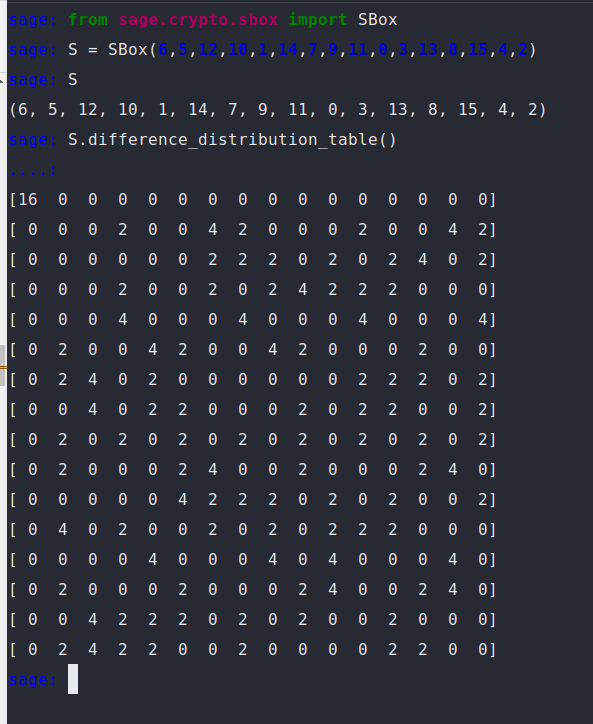
\includegraphics[width=8cm]{img_1.png}
\end{figure}
\textbf{ShiftRow(SR)-}\\
It is the left rotation of the rows of the state matrix.\\
The Rotation offset of each row is given as follows-
\begin{table}[]
\begin{tabular}{ll}
Colums & Offset \\
First  & 1      \\
Second & 2      \\
Third  & 3      \\
Fourth & 4     
\end{tabular}
\end{table}\\

\vspace{10cm}
The LAT is implemented as:

\begin{figure}[htp]
    \centering
    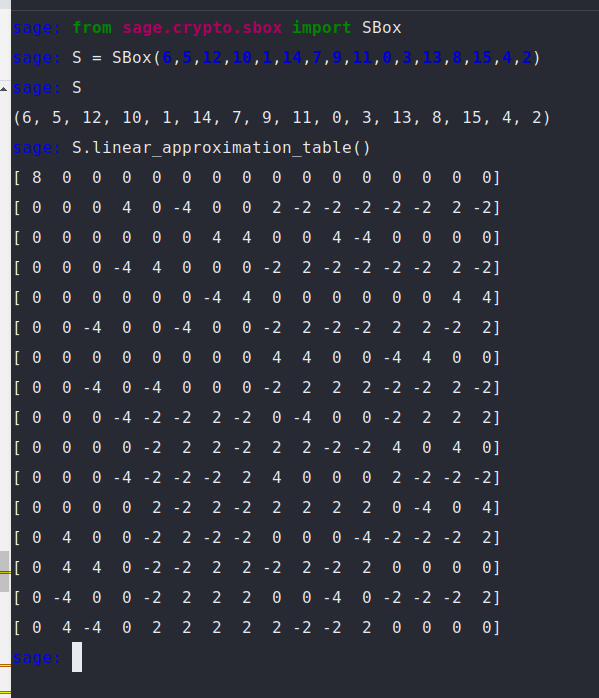
\includegraphics[width=8cm]{img_2.png}
\end{figure}

we get the values of differential branch number and differential uniformity with the help of sage math as:


\begin{figure}[htp]
    \centering
    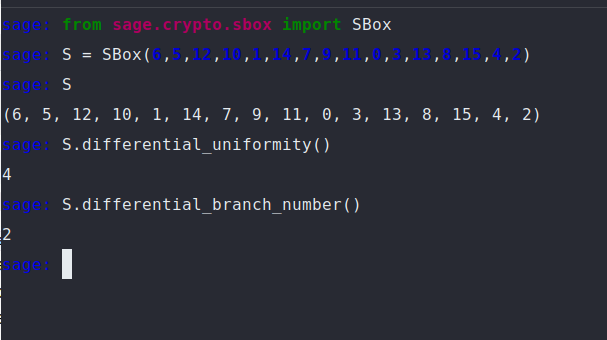
\includegraphics[width=6cm]{img_3.png}
\end{figure}



let's compare the values of the branch number and differntial uniformity of other ciphers with that of ours:

\begin{table}[!ht]
    \centering
    \tiny
    \begin{tabular}{|l|l|l|l|l|}
    \hline
        Group Name & Cipher Name & SBox Size  & Differential Uniformity & Differential Branch Number \\ \hline
        gugu gaga & Midori & 4-bit  & 4 & 2 \\ \hline
        SPL Encrypted  & GIFT & 4-bit & 6 & 2 \\ \hline
        Hope we "3" SDVV & Serpent & 4-bit & 4 & 3 \\ \hline
        -.././cipher  & Prince & 4-bit & 4 & 2 \\ \hline
        TechHeist 3.0 & Pride & 4-bit & 4 & 2 \\ \hline
        Rook & Ascon & 5-bit & 8 & 3 \\ \hline
        Three Amigos & Klein & 4-bit & 4 & 2 \\ \hline
        Decryptor & PHOTON-beetle & 4-bit & 4 & 3 \\ \hline
        cryptoducks & LED & 4-bit & 4 & 3 \\ \hline
        Ping 999+ & Elephant & 4-bit & 4 & 3 \\ \hline
        Kryptonian & Wage  & 8-bit & 8 & 2 \\ \hline
        cipherbytes & Aria & 8-bit & 4 & 2 \\ \hline
        C14 & Primates APE & 5-bit & 2 & 2 \\ \hline
        BitBees & Skinny & 4-bit & 2 & 2 \\ \hline
        Bash Ciphers & PRINT & 3-bit & 2 & 2 \\ \hline
        SHA69 & Mysterion  & 4-bit & 4 & 2 \\ \hline
        Hex Brains & Rectangle & 4-bit & 4 & 2 \\ \hline
    \end{tabular}
\end{table}


\hspace{30cm}
The Differential Branch Number Signifies that the greater the value , the greater the diffusion power of the permutation of SBox.

Our Sbox has the branch number as 2 so its not as much powerful as some of the other ciphers like Serpent , LED etc.


Similarly, differential uniformity tells us the spread of the Sbox . the lower the value the more powerful the Cipher is.\\
Our uniformity value is 4 which is not much powerful but at a mediocre stage than other ciphers.

\textbf{Key Schedule-}\\
 We can have 2 types of keys with different length i.e. 80 or 128 bits\\

\textbf(CASE-1: 80-bit key)\\
If the key is of 80-bit, it is represented as 5x16 rectangular array as shown in the figure below-\\

\begin{bmatrix}
$k_{0,15}$ &...&$k_{0,2}$ & $k_{0,1}$ & $k_{0,0}$ \\
$k_{1,15}$ &...&$k_{1,2}$ & $k_{1,1}$ & $k_{1,0}$\\
$k_{2,15}$ &...&$k_{2,2}$ & $k_{2,1}$ & $k_{2,0}$\\
$k_{3,15}$ &...&$k_{3,2}$ & $k_{3,1}$ & $k_{3,0}$\\
$k_{4,15}$ &...&$k_{4,2}$ & $k_{4,1}$ & $k_{4,0}$
\end{bmatrix}

Key’s 2D Representation\\

Suppose Rowi = $k_{i,15}$|| ... ||$k_{i,1}$|| $k_{i,0}$ indicate the i-th key register’s row, such that 0 $\leq$ i $\leq$ 4, where Rowi is considered to a sixteen bit word. At round i where i belongs to 0 to24, the sixty-four bit round subkey $K_i$ contains the 1st 4 rows of the key register’s contents (as shown in the figure given below), i.e., Ki = Row3 || Row2 || Row1 || Row0.Once the key register Ki found out, the key register gets updated using the following iterations-

\begin{enumerate}
\item We execute Subcoumn to the partial bits that intersect at the four uppermost rows and the four rightmost columns using the S-box S.i.e  i.e., k’3,j || k’2,j || k’1,j || k’0,j := S(k3,j || k2,j || k1,j || k0,j ), such that j belongs to (0, 1, 2, 3).\\
\item Using 1-round generalized Feistel transformation, i.e.,\\
Row'0 := (Row0 << 8) $\oplus$ Row1\\
Row'1 := Row2\\
Row'2 := Row3\\
Row'3 := (Row3 << 12) $\oplus$ Row4\\
Row'4 := Row0\\
\item  Now on the 5-bit key state (i.e. k0,4|| k0,3 || k0,2 || k0,1|| k0,0), we perform a XOR operation with RC[i] (a 5-bit round constant), i.e., k’0,4 || k’0,3 || k’0,2 || k’0,1 || k’0,0 := (k0,4|| k0,3|| k0,2|| k0,1 || k0,0) $\oplus$ RC[i]\\
Using the aforementioned iterations on the revised key state, we ultimately obtain K25. The round constants RC[i] are produced using a 5-bit LFSR for all i between 0 and 24. The five bits (rc4, rc3, rc2, rc1, rc0) are left-shifted by one bit at each round, and the new value of rc0 is then assessed as rc4 xor rc2. At the beginning, RC[0]:= 0x1 is taken. Now that we have it, we can use it to derive all the round constants (for i=0 to 24):  (0X01, 0X02, 0X04, 0X09, 0X12, 0X05,0X0B, 0X16, 0X0C, 0X19, 0X13, 0X07, 0X0F, 0X1F, 0X1E, 0X1C, 0X18, 0X11, 0X03,0X06, 0X0D, 0X1B, 0X17, 0X0E, 0X1D).
\end{enumerate}\\
\textbf(CASE-2: 128-bit key)\\
If the key is of 80-bit, it is represented as 4x32 rectangular array as shown in the figure below-\\

\begin{bmatrix}
$k_{0,31}$ &...&$k_{0,2}$ & $k_{0,1}$ & $k_{0,0}$ \\
$k_{1,31}$ &...&$k_{1,2}$ & $k_{1,1}$ & $k_{1,0}$\\
$k_{2,31}$ &...&$k_{2,2}$ & $k_{2,1}$ & $k_{2,0}$\\
$k_{3,31}$ &...&$k_{3,2}$ & $k_{3,1}$ & $k_{3,0}$\\
\end{bmatrix}
Key’s 2D Representation\\

Suppose Rowi = $k_{i,15}$|| ... || $k_{i,1}$|| $k_{i,0}$ indicate the i-th key register’s row, such that 0 $\leq$ i $\leq$ 4, where Rowi is considered to a sixteen bit word. At round i where i belongs to 0 to24, the sixty-four bit round subkey Ki contains the 1st 4 rows of the key register’s
contents (as shown in the figure given below), i.e., $K_i$ = Row3 || Row2 || Row1 || Row0. Once the key register $K_i$ found out, the key register gets updated using the following iterations-\\
\begin{enumerate}
\item We execute Subcoumn to the partial 8 rightmost column i.e., k’3,j || k’2,j || k’1,j || k’0,j := S(k3,j || k2,j || k1,j || k0,j ), such that j belongs to (0, 1, 2, 3,4,5,6,7).\\
\item Using 1-round generalized Feistel transformation, i.e.,\\
Row'0 := (Row0 << 8) $\oplus$ Row1\\
Row'1 := Row2\\
Row'2 := (Row2 << 12) $\oplus$ Row3\\
Row'3 := Row0\\
\item  Now on the 5-bit key state (k0,4|| k0,3|| k0,2|| k0,1|| k0,0), we perform a XOR operation with RC[i] (a 5-bit round constant), where round constants RC[i] for i belongs to zero to twenty-four are the same used above in the previous 80-bit key schedule. Then finally, we get K25 using the above iterations on the updated key state.
\end{enumerate}


\section{Differential Cryptanalysis}



It is the way where we observe the differences between input plaintexts and relate it to the output differences . It is a kind of strong attack on the Rectangle cipher.\\
We know that to attack a n-bit block cipher using differential cryptanalysis there must be a difference propagation with a probablity significantly larger than $2^{1-n}$ .\\
As the block size is 64 bits . so our cipher must have a difference propagation of at least $2^{-63}$ to be safe from the differential attack . \\
We know from the DDT Table that , the max differential probaility is : $2^{-6}$.\\
The value of differential branch number was = 2 and differntial uniformity = 4.\\

There was a attack generated on the Rectangle cipher for upto 15 rounds . The probability of the trail of 15-rounds was found to be as : $2^{-66}$.\\


\begin{array}{||c|c||c|c||c|c||}
\hline \sharp R & \text { Prob. } & \sharp \mathrm{R} & \text { Prob. } & \sharp \mathrm{R} & \text { Prob. } \\
\hline 1 & 2^{-2} & 6 & 2^{-18} & 11 & 2^{-46} \\
\hline 2 & 2^{-4} & 7 & 2^{-25} & 12 & 2^{-51} \\
\hline 3 & 2^{-7} & 8 & 2^{-31} & 13 & 2^{-56} \\
\hline 4 & 2^{-10} & 9 & 2^{-36} & 14 & 2^{-61} \\
\hline 5 & 2^{-14} & 10 & 2^{-41} & 15 & 2^{-66} \\
\hline
\end{array}


As the ShiftRow Operations of the cipher is simple, the security of Rectangle against cryptanalysis is difficult . \\
Due to rotational symmetry every trail has upto 16 variants . For a 15 round algorithm , the differential probability lies between $2^{-66}$ to $2^{-76}$.\\

So after some experimental data, we get that it is impossible to construct an effective 15 round differential attack (distinguisher) . 4 more rounds are required to attain full dependency. Hence 25 rounds were made fixed for the RECTANGLE cipher to resist the attack . 
















\section{Integral Cryptanalysis}

we apply a 4 round distinguisher attack on the text with the help of two sets of plaintexts,P1 and P2

we assign 0 to the 32nd and 48th value of P1 set plaintexts and assign a 1 to the 32nd and 48th index of P2 set plaintexts.

\begin{figure}[htp]
    \centering
    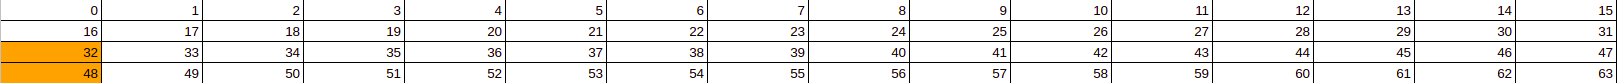
\includegraphics[width=16cm]{img_4.png}
\end{figure}

\begin{figure}[htp]
    \centering
    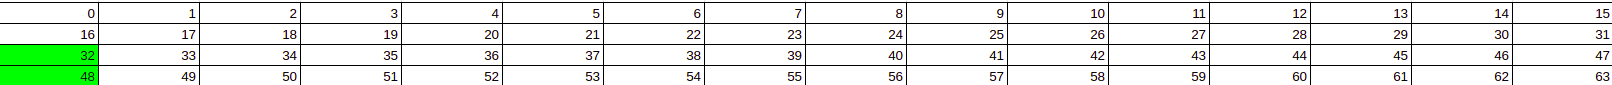
\includegraphics[width=16cm]{img_5.png}
\end{figure}

% \vspace{100cm}
The rest of the blocks are assigned a constant value . i.e a constant property is assigned to the all the rest of the blocks in both of the sets.\\
so now we can basically see that the difference of the blocks is non-zero in the 0th column while its 0 for all the leftover columns\\
so therefore we can infer that :\\
P1(col0) $\oplus$ P2(col0) = 1100\\
Let's see the encryption part:\\
as we apply the encryption on plaintexts, we see that after 4 rounds of encrpytion the only places that are left with 0 output difference is the postion number 0 , 17,43 and 60.\\
which means that the position 0,17,43,60 accept the balanced property. \\


% \vspace{20cm}
\begin{figure}[htp]
    \centering
    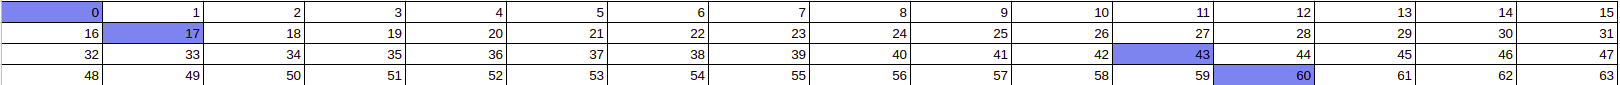
\includegraphics[width=16cm]{img_6.png}
\end{figure}


\vspace{1cm}
Let's see how we can do the decryption on the given set of texts,\\
we take $2^{48}$ plaintexts such that the columns 0 , 13 , 14 ,15 contains a fixed constant value and other blocks have a All property.\\

\begin{figure}[htp]
    \centering
    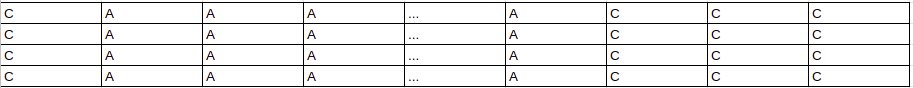
\includegraphics[width=12cm]{img_7.png}
\end{figure}

After encrypting 3-rounds $2^{48}$ values can be divided into $2^{47}$ subsets where each subset contains two values satisfying the above 4-round.\\
This can be don upto 7 rounds of encryption .\\
But as 25-round Rectangle provides sufficient security against the Integral Cryptanalysis.

\vspace{10cm}
\section{Software Implementation}
We have implemented Rectangle cipher on 64-bit operating system with a python interpreter.\\
\textbf{Cipher Implementation: }\\
We have designed RECTANGLE cipher for vector 4 16-bit words,and a key vector of 5 16-bit word.\\
We are taking input in hex format and printing it into binary format\\
If input have less than 64 bits then padding of 0 is added in the end.\\
Alongwith that a decryptor function that takes input as ciphertext and key  is also made which returns us the plaintext back .

\textbf{Below are the screenshots of the terminal-}\\

\begin{figure}[htp]
    \centering
    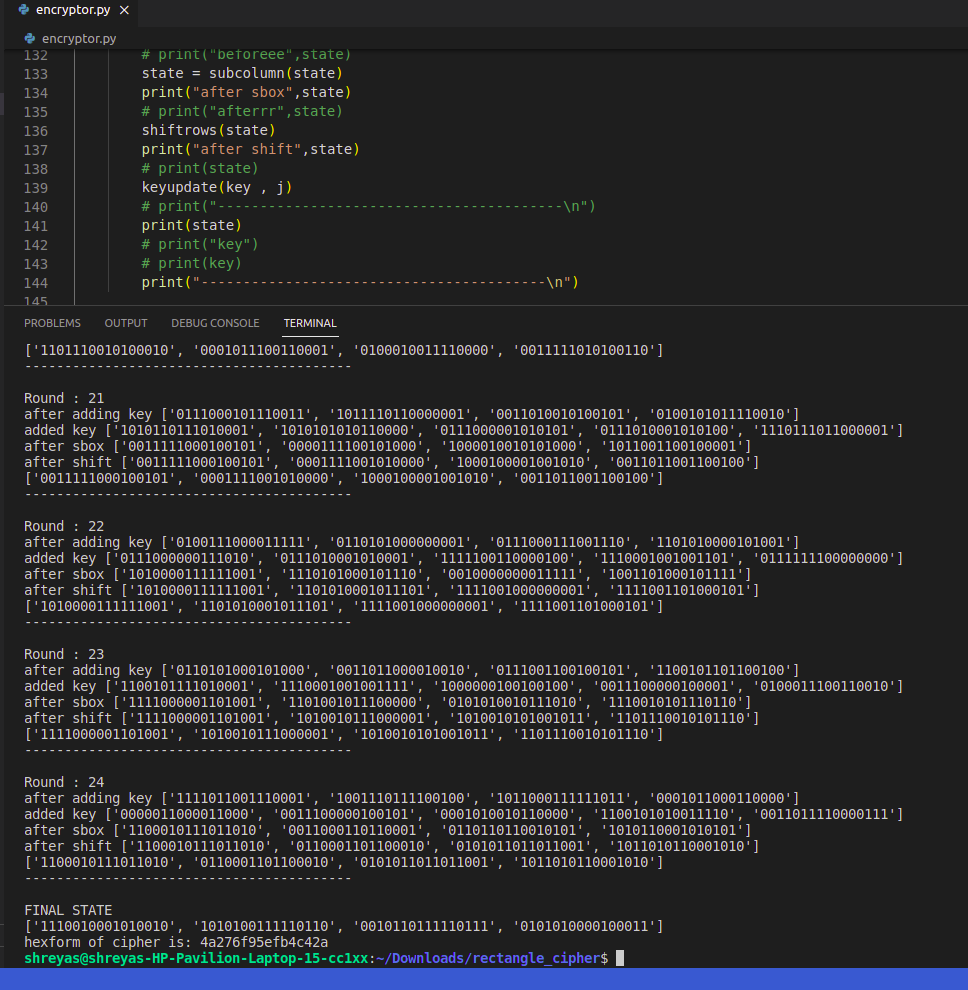
\includegraphics[height=10cm]{img_11.png}
\end{figure}


\begin{figure}[htp]
    \centering
    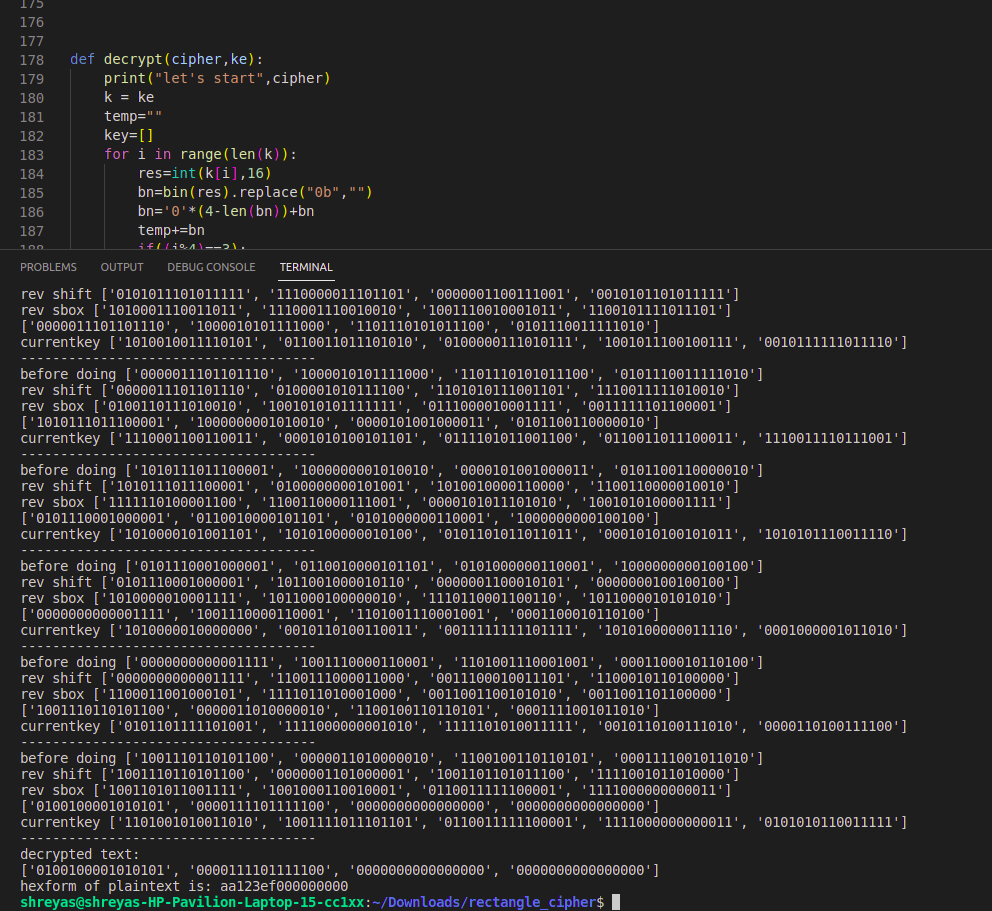
\includegraphics[width=10cm]{img_12.png}
\end{figure}


\vspace{15cm}
\textbf{Software Implementation-}\\
Software Implementation contains 3 files-
\begin{enumerate}
    \item server.py-opens socket and waits for the client to connect and share message.
    \item client.py-establishes connection i.e binds with socket of server.py
    \item encryptor.py-contains the encryption of the RECTANGLE cipher
    \item decryptor.py- contains the decryption of the RECTANGLE cipher
\end{enumerate}\\

We have implemented a client server based application in which client can send a messsage to server in the form of UDP packets and server in return sends the encrypted message which also is in the form of UDP packet.\\
key is kept secured with the server which no client can access it.\\
Server here acts as a black box or oracle for each and every client which establishes a connection with server.\\
\textbf{Below are the screenshots of the terminal-}\\

\begin{figure}[htp]
    \centering
    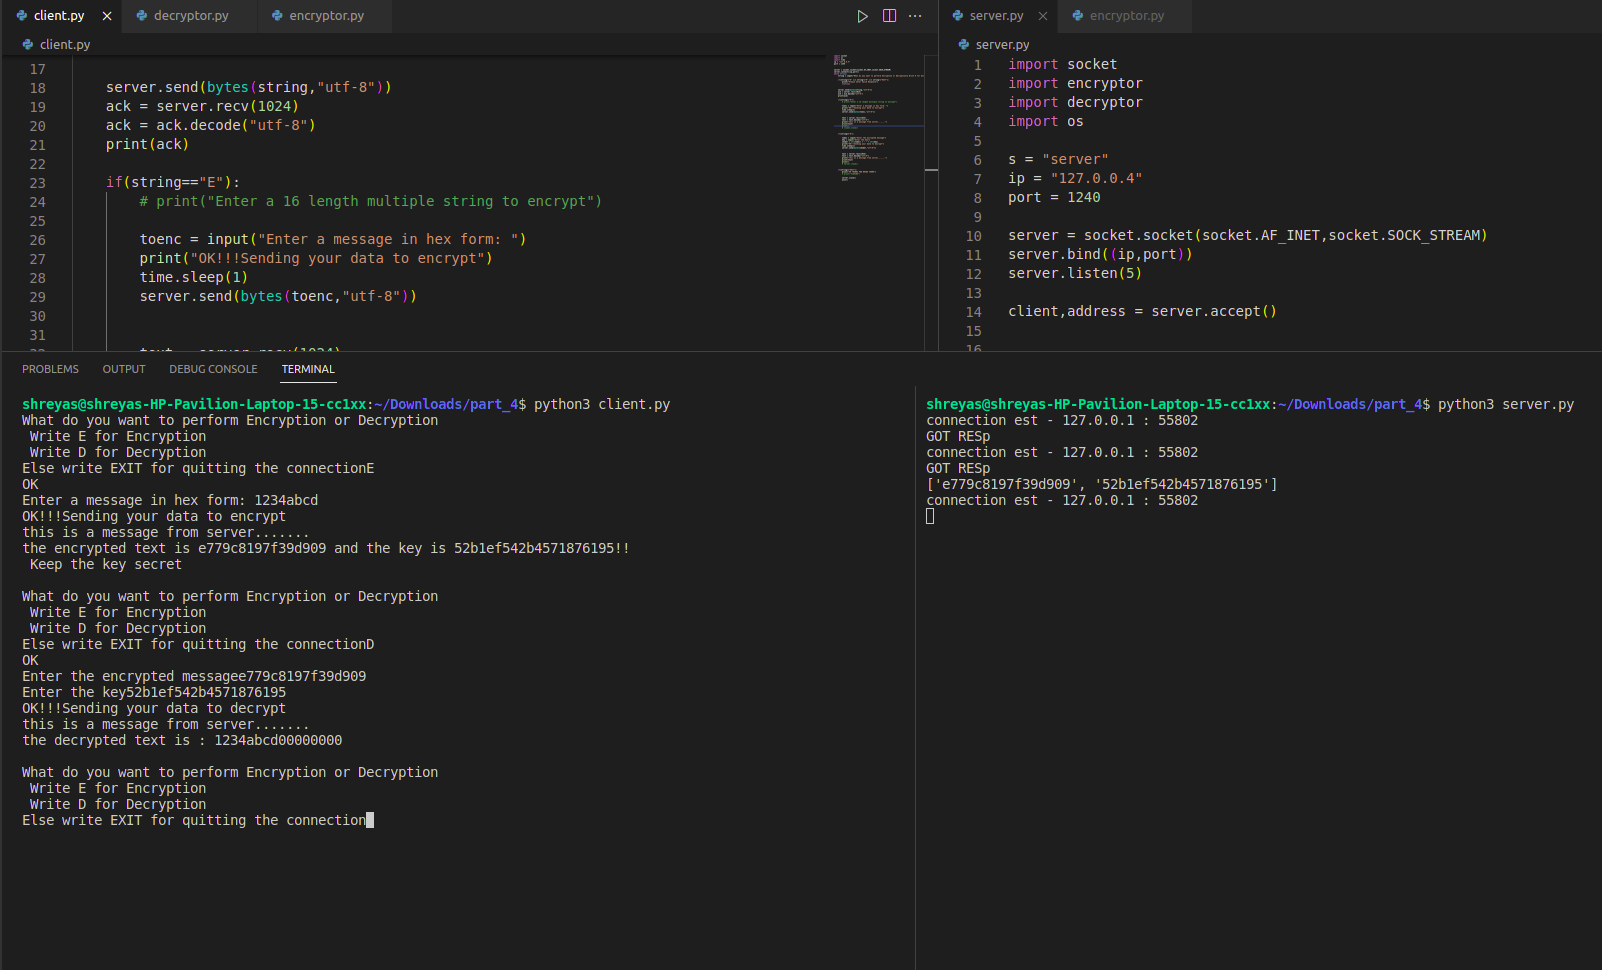
\includegraphics[width=10cm]{img_10.png}
\end{figure}


\vspace{10cm}
\section{Conclusion}
A bit-slice approach based on SP-Network has been presented as part of RECTANGLE, a lightweight block cypher that is quick to execute. Both a highly quick and competitive software performance and a very affordable hardware performance are attained. In the parallel substitution layer, there are 16 44 S-Boxes, and in the permutation layer, there are 3 rotations. Excellent hardware and software performance is offered by rectangle. in order to provide applications with sufficient flexibility.Because to the careful selection of the cipher's Substitution box and the asymmetric architecture of the permutation layer, Rectangle achieves a higher security performance. The Rectangle cypher is said to be a straightforward and intriguing design with the potential to lead to numerous new cryptographic issues. Rectangle cypher security is thereafter advocated.

\section{References}
\begin{enumerate}
    \item https://eprint.iacr.org/2014/084.pdf
    \item https://eprint.iacr.org/
\end{enumerate}

%%%% 8. BILBIOGRAPHY %%%%

\bibliographystyle{alpha}
\bibliography{abbrev3,crypto,biblio}
%%%% NOTES
% - Download abbrev3.bib and crypto.bib from https://cryptobib.di.ens.fr/
% - Use bilbio.bib for additional references not in the cryptobib database.
%   If possible, take them from DBLP.

\end{document}
